\documentclass[acmtog, authorversion]{acmart}

\usepackage{booktabs} % For formal tables
\usepackage{hyperref}

% TOG prefers author-name bib system with square brackets
\citestyle{acmauthoryear}
\setcitestyle{square}

\usepackage[ruled]{algorithm2e} % For algorithms
\renewcommand{\algorithmcfname}{ALGORITHM}
\SetAlFnt{\small}
\SetAlCapFnt{\small}
\SetAlCapNameFnt{\small}
\SetAlCapHSkip{0pt}
\IncMargin{-\parindent}

% Metadata Information
\acmYear{2017}
\acmMonth{9}

% Copyright
%\setcopyright{acmcopyright}
%\setcopyright{acmlicensed}
\setcopyright{rightsretained}
%\setcopyright{usgov}
%\setcopyright{cagov}
%\setcopyright{cagovmixed}

% Document starts
\begin{document}
% Title portion
\title{Finding trends in open-source software by visualizing collaboration and influence over time} 

\author{Rick Proost}
\affiliation{%
  \institution{Delft University of Technology}
  \country{The Netherlands}}
\email{rpjproost@gmail.com}

\author{Vincent Robbemond}
\affiliation{%
  \institution{Delft University of Technology}
  \country{The Netherlands}}
\email{vincentrobbemond@gmail.com}

\author{Wim Spaargaren}
\affiliation{%
  \institution{Delft University of Technology}
  \country{The Netherlands}}
\email{wim_spaargaren@live.nl}

\begin{abstract}
Since the open-source software community has seen such enormous growth in past years and remains to grow still, a wealth of data has become available.
Collaboration platforms like GitHub provide easy access to all open-source project data by providing an API.
While this data has been available for some time, there has not been done a lot of research into how this data can be applied to bring insights in the way developers collaborate.
Developer collaboration has become a bigger point of discussion since the rise of Globally Distributed Software Engineering and can benefit from insights derived from this readily available data.
This paper describes the building of an online platform to provide open source software collaboration visualizations on GitHub.
In addition, the evolution of developer activity for open source software projects  is explored.
This exploratory research is done by answering questions about the evolution of developer activity in the developer community and the amount of commits made by a developer per country.
\end{abstract}

\keywords{Data Visualization, GitHub, Open Source Software, Collaboration}

\maketitle

\section{Introduction}
In the past few years the open-source software(OSS) community and development in OSS have grown enormously.
According to GitHub \cite{GHOctoverse}, in 2016, there were over 5.8 million users engaged in activities relating to public repositories.
GitHub defines these activities as "some activity within the last year, e.g. code committed, a comment created, a repository starred, or an issue opened".

With GitHub providing programmatic access to all OSS repository and user data\cite{GHAPI}, it is possible to collect and manipulate this data to get more insights into the way the OSS community collaborates (on GitHub).
These new insights can then be applied to to e.g. develop new software development methods, improve existing (collaboration) platforms (like GitHub) or coding standards, which improve developer collaboration \cite{Jermakovics2013}.
Outside of the OSS community, a better understanding of how the OSS community functions helps commercial IT projects adopt typical OSS practices, e.g. promoting open collaboration \cite{Kalliamvakou:2015:OSC:2818754.2818825}, and may help IT planners make more informed decisions and develop more effective strategies for using OSS software \cite{madey2002}. 

One way for researchers to analyze the gathered data, is by visualizing it \cite{Heller}.
One of the objective of the Software Visualization field is to aid stakeholders in developing a greater understanding of software systems, their evolution and development.
"The basic idea of visual data exploration is to present the data in some visual form, allowing the human to get insight into the data, draw conclusions, and directly interact with the data. 
Visual data mining techniques have proven to be of high value in exploratory data analysis and they also have high potential for exploring large databases." \cite{981847}.
To give developers insights in repositories, GitHub also provides some visualizations, one of these visualization is "Developer Contribution", which shows amount of commits made during a period of time.
Up until now there have not been a lot of tools or platforms which provide visual insight into e.g. collaboration over time on a specific repository.
Tools which are available are outdated \cite{Heller} or not sufficient, for example a visualization of GitHub's newest and most popular repositories \cite{donnemartin2016}, a GitHub repository history visualizer \cite{artzub2013}, and a repository stats visualizer \cite{bajaj2013}.
Although these examples are visualization tools for GitHub, they provide insufficient information on developer collaboration in OSS projects.

Therefore, the aim of this paper is to provide a tool/platform which stakeholders can leverage to gain insights into OSS projects and developer collaboration.
For example, making this data available can show where developers are located, this in turn helps identifying possible cultural differences between collaborators which is important to prevent co-ordination and collaboration problems \cite{Mishra2014}.
Such a tool or platform could be really helpful in the field of software engineering.

The research question this paper will try to answer is: \textbf{Is it possible to find different patterns in OSS development by visualizing collaboration over time?}

Since this is a broad subject, we will explore this subject by answering a number of questions.
However, these answers will not provide a conclusive answer to the main question asked but in turn invite others to extend and explore this subject.
In total, two sub questions will be answered, focusing on more specific patterns.
The first possible trend could emerge by analyzing the active number of developers in the OSS community per country.
This trend is expected because the amount of developers per country differs as stated in \cite{StackOverflow2017}.
By adding a temporal element to active number of developers per country, it might be possible to tell in which countries the number of active developers in open-source software evolves faster.
This could be interesting to know for companies seeking open-source developers to outsource software development to \cite{haefliger2008code}.

Underlying reasons can then be researched for this rise in popularity.

Therefore we first aim to answer the question: \textbf{Does the number of active developers in the OSS community evolve faster for different countries?}

Another possible trend could emerge in collaboration links for projects.
Collaboration links are defined as links between developers who add contributions consecutively to the same project.
By adding a temporal component to visualizing collaboration links, it becomes possible to see the way developer collaboration changes over time.
At the same time it becomes possible to see if the distance between developers working on the same project has influence on collaboration.

The second question we aim to answer is: \textbf{Does the number of commits made by a developer evolve faster for different countries?}

The answers could be derived from visualizing the data in such a way researchers can make well substantiated and testable hypotheses. 
Therefore, the main outcome is that a service was developed that visualizes evolution on collaboration over time for development.

\section{Methodology}
To answer these questions a set of large repositories (i.e. repositories with the most GitHub stars and/or collaborators) on the open source software platform GitHub have been chosen.
A crawler is built to retrieve data from the above mentioned repositories.
The crawled data includes (but is not limited to) the owner, contributors and collaborators of the repository.
Aside from user information, commits are gathered for the repositories to compare statistics in different time frames.

A web-based service is created to quickly search and navigate repositories or GitHub users.
Data gathered can then be displayed in multiple forms like geolocations for collaborators on an interactive map (e.g. Mapbox \cite{MapBox}) and activity for a project in a graph with a temporal component.
Different ways of linking users and repositories is experimented with and results are published and available online at \url{https://github.com/VincentRbbmnd/in4334-sa-report}.

By creating this web-based service, new insights will emerge for collaboration in open source software development.
Trends in software collaboration, activity and collaboration links over time will be revealed.
Besides the answers to these questions a new way is provided for researchers to get visual insights in open source software development collaboration statistics and form new hypotheses.

\section{Implementation}
The first step in finding answers to the research questions, is to gather data from the software development platform GitHub. 
This data is gathered by using the GitHub REST API\cite{GHAPI}. 
The gathered repositories limits to the top 1000 starred repositories on GitHub, for two reasons:
First, according to Octoverse \cite{GHOctoverse} in 2016 there were nearly 20 million software repositories, storage of this amount of data goes beyond the scope of this research paper.
The second reason to choose the most starred repositories, is that users of GitHub star a repository when they think the repository is interesting and/or are a collaborator for that repository).
 
Because of this it was decided to use only the top 1000 most starred GitHub projects specified at \url{https://gitstar-ranking.com/} at september 2017. 
Data for these projects was gathered by building a custom crawler in Golang, which stores the data in a Postgres database and can be run as cron job which be continuously scanning the GitHub API for project changes.
First project data is gathered using the projects resource\cite{GHAPI}.
After the project data was gathered, the commits resource\cite{GHAPI} was used to gather all commits for the collected projects. 
This was done by crawling all paginated requests for commits per Project. 
Commit data contains a message which is mostly used to describe the change and a timestamp denoting commit time.
Commit author and committer data is also available, so it is possible to make this distinction.
This user data was also stored in a separate table.
Finally, star data was gathered from the repository stargazer resource\cite{GHAPI}.
A stargazer is a user who starred a certain repository, so Developer A stars Repository B, therefore A is now in the list of stargazers of B.
By adding a custom header to this API request it was possible to retrieve the timestamp for when the user starred the repository.
This way it was possible to find which user starred a project at what time.
A second cron job was written to find locations for users. 
The GitHub platform allows a user to specify a location on their profile, which is stored as plain text.

However to use these locations, coordinates are needed. 
To transform these locations to coordinates the Google Places API was used. 
This way coordinates were found for all specified locations on which the Google Places API returns coordinates.

\section{Results}
The self developed crawler can be found at \url{https://github.com/VincentRbbmnd/in4334-sa-report} and will keep gathering data to make sure our database stays up to date with the current state of the GitHub platform.

\begin{figure}
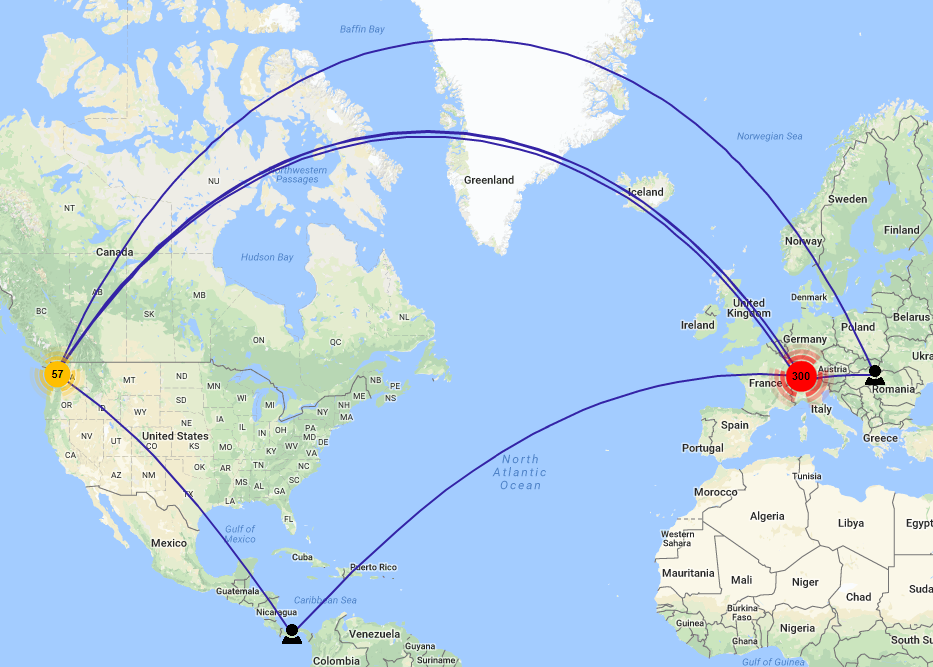
\includegraphics[scale=0.3]{visualizer-example.PNG} 
\caption{Example visualization of developer collaboration (early stage version)}
\label{fig:collaboration}
\end{figure}

Figure ~\ref{fig:collaboration} shows an example of an early stage visualization in the process of building the visualizer.
Here, nodes depict developers and lines depict collaboration between developers.
When at a lower zoom level, nodes get un-grouped and lines between individual developers will be shown.

\begin{figure}
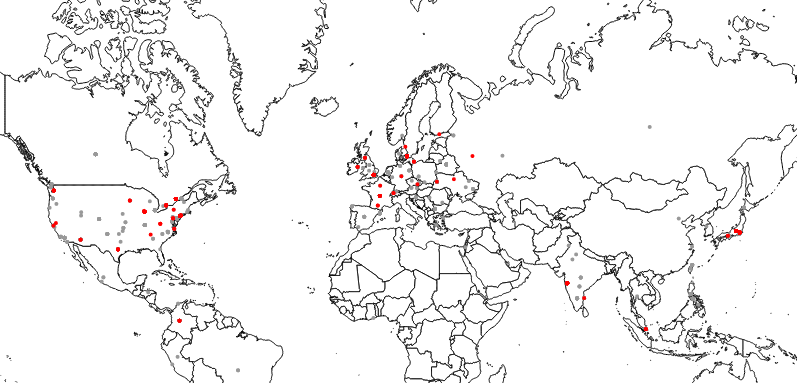
\includegraphics[scale=0.4]{d3-example-rails.PNG} 
\caption{Example visualization of commits during a certain time period}
\label{fig:commits-period}
\end{figure}

Figure ~\ref{fig:commits-period} shows an example of a map built with the D3 library, with all dots representing commits belonging to a repository, with the red dots representing commits made during a selected period of time.

Preliminary results contain 1000 repositories with over 5 million commits belonging to 160.000 users. 
Not all of the user gave information on their whereabouts, but about 84.000 did.
This means that it was possible to retrieve locations for just over 50\% of the gathered users.

\bibliographystyle{ACM-Reference-Format}
\bibliography{bibliography}

\end{document}

